\documentclass{article}

\usepackage[utf8]{inputenc}
\setlength{\parindent}{0em}
\setlength{\parskip}{1em}
\usepackage[T1]{fontenc}  

\usepackage{graphicx, graphics, amsmath, amssymb, xcolor, mathtools, bbm, mathabx} % deleted asmthm because of conflict with already existing 'proof' environment
\usepackage{siunitx}

\usepackage{subcaption}
\usepackage{stmaryrd}

\usepackage{tabularx}
\usepackage{array}
\usepackage{changepage}
\usepackage{setspace}
\usepackage{tcolorbox}
\usepackage{mathtools}
\DeclarePairedDelimiter\floor{\lfloor}{\rfloor}

\newenvironment{proof}
{\textbf{Proof:} \hspace{10pt}} % begin code
{\hfill{$\Box$}} % end code

\newcounter{example}

\newenvironment{example}[0]% environment name
{% begin code
  \newline
  \newline
  \refstepcounter{example}%
  \textbf{Example \theexample} \hspace{10pt}
}%
{\hfill \newline \newline% end code
}

\newtheorem{stelling}{Stelling}

\usepackage[labelfont=bf, labelsep=colon, format=hang, textfont=singlespacing]{caption}

\usepackage{booktabs}% for \midrule and \cmidrule macros
\newcommand\headercell[1]{%
   \smash[b]{\begin{tabular}[t]{@{}c@{}} #1 \end{tabular}}}

\DeclareMathOperator*{\argmax}{arg\,max}
\DeclareMathOperator*{\argmin}{arg\,min}

\newcommand{\norm}[1]{\left\lVert#1\right\rVert}

\title{Bachelorproef Semester 2}
\author{Nina van der Bruggen \& Ilias Willems}
\date{February 2021}

\begin{document}

\maketitle

\tableofcontents

\newpage

\begin{abstract}
    It is no exaggeration to state that least squares regression has been, and continues to be, one of the crown jewels of statistics. However, it is not a silver bullet for all problems: sometimes it lacks the necessary prediction power or cannot be computed at all. In these cases other methods are required. In this paper we introduce, motivate and explain ridge and Lasso estimation and provide a comparison between the two by applying them on a data set, as well as a comparison between them and regular least squares regression. For the comparison, we use a technique called Cross-Validation, which we will also explain in detail.
\end{abstract}
\section{Introduction}
In a first part of this paper, we explain regular least squares regression in a nutshell, introducing the necessary notations for the rest of the paper. In this discussion we also point out two problems with the method:
\begin{itemize}
    \item \textit{Prediction accuracy}: If $n \gg p$, then least squares fitting will have low variance. However, if $n$ is not much larger than $p$, least squares fitting tends to have high variance (overfitting). If $p > n$, then the variance is even infinite.
    \item \textit{Model interpretability}: Removing unnecessary variables from the model improves the interpretablility of the result.
\end{itemize}
The solution to the first problem will lead us the ridge estimator. We will analyze, both theoretically and 
\newpage
\section{Penalized Regression} \label{sec:3.PR}
Linear regression is a simple and elegant method for analysing data and constructing models that can be used to make predictions. It is an unbiased estimator and therefor belongs to the class of linear unbiased estimators. Moreover, the theorem of Gauss-Markov~\cite{SIDA2021} tells us that it is the best estimator in its class, which means that its variance is smaller than any other linear unbiased estimator. Unfortunately, there are some problems that arise in certain situations which makes linear regression very bad (i.e. the variance of the coefficients is very high) or even impossible. The solution to these problems give rise to a different class of estimators, called the Bridge estimators~\cite{WWM2020}. This class contains infinitely many estimators, but we will focus on two special cases, called the ridge and Lasso estimators.\\
\\
In this section we will first investigate these problems with linear regression and illustrate them with some code in $R$. Solving these issues will lead us in a very natural way to the ridge and lasso estimators, for which we will also provide illustrations using $R$. We will find that we can fine-tune these estimators further by selecting the right \textit{tuning parameter} $\lambda$. To do this we will need a method to compare different models, which we will address in section~\ref{sec:4.CV&PS}. Finally, we compare the ridge and lasso estimators in section~\ref{sec:5.CRL}.

%----------------------------------------
% --- Linear regression and its flaws ---
%----------------------------------------

\subsection{Linear regression and its flaws} \label{sec:1.1.LR}
Suppose we make observations of $p+1$ variables. Our aim is to predict one of these variables, called the \textit{target}, based on the other $p$ variables, called the \textit{predictors}. If we make $N$ observations, we can construct a \textit{data matrix }
\begin{equation*}
    \textbf{X} = \begin{pmatrix}
    1 & x_{11} & x_{12} & \dots & x_{1p}\\
    1 & x_{21} & x_{22} & \dots & x_{2p}\\
    \vdots & \vdots & \vdots & \ddots & \vdots\\
    1 & x_{N1} & x_{N2} & \dots & x_{Np}
    \end{pmatrix}
\end{equation*}
that contains the predictors of the $i$'th observation in its $i$'th row and  where we added a column of ones in the front. This column of ones will be useful later when we want to calculate the intercept of the regression line. Similarly, we can construct a vector of the targets, called the \textit{target vector}
\begin{equation*}
    \textbf{y} = \begin{pmatrix}
    y_1\\
    y_2\\
    \vdots\\
    y_N
    \end{pmatrix}.
\end{equation*}
The problem now is to find a vector $\beta$ such that $\textbf{X}\beta$ is 'as close as possible' to the target vector \textbf{y}. To this end, we want to minimize the \textit{residual sum of squares (RSS)} defined as
\begin{equation*}
    \textrm{RSS}(\beta) = \sum_{i=1}^N (y_i - \textbf{X}_i \beta)^2
\end{equation*}
where $\textbf{X}_i$ denotes the $i$'th column of $\textbf{X}$, or in matrix notation
\begin{equation*}
    \textrm{RSS}(\beta) = (\textbf{y} - \textbf{X}\beta)^T(\textbf{y} - \textbf{X}\beta).
\end{equation*}
It can be shown~\cite{SIDA2021} that the vector $\hat{\beta}$ that minimizes this expression is
\begin{equation}\label{eq:LSSest}
    \hat{\beta} = (\textbf{X}^T\textbf{X})^{-1}\textbf{X}^T\textbf{y}.
\end{equation}
As mentioned before, the Gauss--Markov theorem tells us that the least squares estimator $\hat{\beta}$ is the one with the smallest variance among all linear unbiased estimators of $\beta$. A first problem with this method of regression is immediately obvious from equation~\ref{eq:LSSest}: What if $\textbf{X}^T\textbf{X}$ is not invertible? This is for example always the case if $p > N$. Furthermore, if $n \approx p$ then the variance of $\hat{\beta}$ will be very large. We illustrate this with a simple example.
\begin{example}
We use the \textit{Hitters} data set of the \textit{ISLR} package in $R$. The code used in this example can be found in \textbf{nog te bepalen}.\\
\\
Firstly, we calculate the regression coefficients using almost all the data available ($250$ observations). The mean squared prediction error can be found in Table~\ref{tab:exampleLSS}. In the next step, we restrict the data we use to the first $100$ observations, apply linear regression on the restricted data and store the mean squared prediction error of the regression parameters in Table~\ref{tab:exampleLSS} below. This process is then repeated for data sets of $75$, $50$, $25$ and $10$ observations.
\begin{table}[ht]
    \centering
    \begin{tabular}{c|c}
         Sample size & Mean Squared Error\\
         \hline
         $250$ & $135825.5$\\
         $100$ & $136102.8$\\
         $75$ & $150103.6$\\
         $50$ & $158626.9$\\
         $25$ & $182158.5$\\
         $10$ & $301629.5$
    \end{tabular}
    \caption{Table of the mean squared errors of some least squares models computed with different amounts of data.}
    \label{tab:exampleLSS}
\end{table}
The general trend of the test errors shown in Table~\ref{tab:exampleLSS} is that they increase as the sample size decreases. If the number of observations gets close to the number of predictors, prediction errors get so large that the model will not be able to accurately predict target values based on observations.\\
\\
One could remark that even when using $250$ data points to compute the model, the test error is still quite large. This can be explained by the nature of the values we are trying to predict. The salary of the baseball players lies mostly in the $400-1000$ range, with some outlier values as low as $<90$ and as high as $>2000$. As a consequence, the variance of the data is high: it takes on the value $204243.4$. Having a mean squared error of $135825.5$ means that, on average, our estimates are about $370$ too low or too high. Given the circumstances, one could argue that this is not too bad.
\end{example}

The reason for the test error in the previous example is that if $n \approx p$, linear regression tends to overfit the data. Even though it is unbiased, little knowledge about the data can be acquired from this model. We say that in these cases, the model has bad \textit{prediction accuracy}. A similar effect can be observed if the predictor variables are (highly) correlated.\\
\\
A second issue with linear regression is that it takes all variables into account. Especially if the number of predictors is high and there is reason to believe some of them may have nothing to do with the target values\footnote{In a medical study, for example, it would be very reasonable to suspect that the predictor "favorite colour" has nothing to do with the target "suffers from heart decease".}, a desired property of regression would be that the coefficients of these 'useless' predictors are zero. This way we can leave them out of the model, thus reducing the complexity of the model, making it easier to understand and interpret.\\
\\
Both of the issues we just laid out have straightforward solutions: in order to reduce overfitting, we could restrict the size of the coefficients by penalizing large values of $\hat{\beta}$ and in order to make the model more interpretable, we could leave out some predictors. Both of these solutions do come at a cost, namely that they introduce some bias into the model. It can be shown, however, that these solutions do lead to a better model as the small sacrifice in bias leads to a giant decrease of variance, increasing the prediction accuracy of the model. This phenomenon is known as the \textit{bias-variance trade-off}.

%----------------------------------
%-------- Ridge regression --------
%----------------------------------

\subsection{Ridge regression} \label{sec:RidgeRegression}
We will work out the ideas at the end of the previous section mathematically. This will lead to what is known as ridge regression.\\
\\
As we already pointed out, we can reduce the overfitting present in regular linear regression by imposing a size constraint on the coefficients. For this we need to be able to measure the \textit{size} of the vector of coefficients $\hat{\beta}$. There are many ways to measure the size of a vector $\textbf{x}$ in mathematics but we will focus on just two of them, namely the $L_1$ and $L_2$ norm, which are defined as follows:
\begin{equation} \label{eq:L1Norm}
    L_1: \hspace{3pt} \norm{\textbf{x}}_1 = \sum_{i=1}^n |x_i|
\end{equation}
\begin{equation} \label{eq:L2Norm}
    L_2: \hspace{3pt} \norm{\textbf{x}}_1 = \sum_{i=1}^n x_i^2
\end{equation}
The $L_1$ norm given in equation~\eqref{eq:L1Norm} will give rise to the Lasso regression, while the $L_2$ norm given in equation~\eqref{eq:L2Norm} will give rise to ridge regression. It is this last one on which we will focus first.\\
\\
The aim is now to calculate
\begin{equation} \label{eq:Ridge}
    \begin{aligned}
        \hat{\beta}{}^{\text{ridge}} = \argmin_{\beta}\bigg\{\sum_{i=1}^N \bigg(y_i - \beta_0 - \sum_{j=1}^p x_{ij}\beta_j\bigg)^2\bigg\} \newline \text{, subject to } \sum_{i=1}^p \beta_i^2 < t
    \end{aligned}
\end{equation}
which is just regular regression, but with the added size constraint on the coefficients. It can be shown that we can rewrite expression~\eqref{eq:Ridge} to
\begin{equation}\label{eq:RidgeAlt}
        \hat{\beta}{}^{\text{ridge}} = \argmin_{\beta}\bigg\{\sum_{i=1}^N \bigg( y_i - \beta_0 - \sum_{j=1}^p x_{ij}\beta_j\bigg)^2 + \lambda \sum_{i=1}^p \beta_i^2\bigg\}
\end{equation}
where $\lambda$ is called the complexity or tuning parameter. The statistician needs to determine the correct value of $\lambda$ to obtain the best model (i.e. the model with the highest prediction accuracy). This can be achieved using a technique called \textit{Cross-Validation}, which we will explain in a later section. It can be shown that the parameter $t$ in equation~\eqref{eq:Ridge} and $\lambda$ in equation~\eqref{eq:RidgeAlt} are in a one-to-one correspondence. Calculating $t$ when $\lambda$ is given is straightforward because $t = \norm{\hat{\beta}{}^{\textrm{ridge}}}^2$. Calculating $\lambda$ for a given $t$ is more difficult. One approach would be to perform ridge regression for a range of values for $\lambda$, then calculate the square of the norm of the regression coefficients and pick the model for which $\norm{\hat{\beta}{}^{\textrm{ridge}}}^2$ is closest to $t$. Another approach could be to start with an initial guess $\lambda_0$, perform ridge regression and calculate $t_0 = \norm{\hat{\beta}{}^{\textrm{ridge}}}^2$. If $t_0 < t$ ($t_0 > t$), choose $\lambda_1 < \lambda_0$ ($\lambda_1 > \lambda_0$) and repeat the process. For this second method we would also need to correctly determine the step length at each step as well as an appropriate error tolerance to ensure the algorithm converges. 

Notice in expressions~\eqref{eq:Ridge} and~\eqref{eq:RidgeAlt} that the penalization term does not involve the intercept $\beta_0$. This is usually a desired property, as penalization of the intercept would make the procedure dependant on the origin chosen for $\textbf{y}$. That is, if we would shift $\textbf{y}$ in some direction by adding a constant $c$ to its components, then this would not simply result in a shift of the predictions by the same amount $c$. We also remark that, like regular regression, ridge regression is sensitive to scale changes. It is therefor advisable to always standardize the data before applying ridge regression.\\
\\
After writing equation~\eqref{eq:RidgeAlt} using matrices $\textbf{X}$, $\textbf{y}$ and $\beta$ as we did in Section~\ref{sec:1.1.LR}, it is not hard to show that
 \begin{equation} \label{eq:ridgeCoef}
    \hat{\beta}{}^{\textrm{ridge}} = (\textbf{X}^T\textbf{X} + \lambda\textbf{I})^{-1}\textbf{X}^T\textbf{y}.
\end{equation}
Important to note here is that the equation above will penalize the intercept if we take our data matrix as we did in Section~\ref{sec:1.1.LR}, namely
\begin{equation*}
    \textbf{X} = \begin{pmatrix}
    1 & x_{11} & x_{12} & \dots & x_{1p}\\
    1 & x_{21} & x_{22} & \dots & x_{2p}\\
    \vdots & \vdots & \vdots & \ddots & \vdots\\
    1 & x_{N1} & x_{N2} & \dots & x_{Np}
    \end{pmatrix}.
\end{equation*}
The column of ones in front is added to calculate the intercept $\beta_0$ automatically, but doing so causes it to be penalized. If this property is not desired, one could opt to not add the column of ones in front of the data matrix, then apply equation~\eqref{eq:ridgeCoef} to get the regression coefficients $\beta_1, \dots, \beta_p$ and calculate the intercept $\beta_0$ separately as, for example, the mean of the target vector.\\
\\
The attentive reader may wonder if the matrix inverse in equation~\eqref{eq:ridgeCoef} always exists. We will prove below that this is indeed the case~\cite{Kj2018}. This means that, contrary to regular regression, we can apply ridge regression in cases where $n < p$.\\
\\
\begin{proof}
    Remark firstly that a matrix of the form $\textbf{X}^T\textbf{X}$ is always positive semidefinite. This can be seen as follows:
    \begin{equation*}
        z^T\textbf{X}^T\textbf{X}z = (\textbf{X}z)^T \textbf{X}z = \norm{\textbf{X}z}_2 \geqslant 0
    \end{equation*}
    The eigenvalues of a positive semidefinite are always bigger than or equal to zero. We show this with a similar argument. Let x be an eigenvalue of a positive semidefinite matrix $\textbf{M}$ with eigenvalue $\gamma$. Then we have:
    \begin{equation*}
        0 \leqslant x^T\textbf{M}x = x^T \gamma x = \gamma \norm{x}_2
    \end{equation*}
    Because $\norm{x}_2 > 0$ if $x \neq 0$ (which is not the case as $x$ is an eigenvector) it follows that $\gamma \geqslant 0$. It is easy to show that if $\gamma$ is an eigenvalue of $\textbf{X}^T\textbf{X}$, then $\gamma + \lambda$ is an eigenvalue of $\textbf{X}^T\textbf{X} + \lambda \textbf{I}$. If $\lambda > 0$, all eigenvalues of $\textbf{X}^T\textbf{X} + \lambda \textbf{I}$ will be strictly positive, so the matrix is invertible.
\end{proof}

% - Theoretical comparison with regular regression -

\subsubsection{Theoretical comparison with regular regression}
To get more insight into formula~\eqref{eq:ridgeCoef}, we compare it to the formula for computing the regular regression coefficients, given in equation~\eqref{eq:LSSest}. For this discussion, we choose to work with the data matrix
\begin{equation*}
    \textbf{X} = \begin{pmatrix}
    x_{11} & x_{12} & \dots & x_{1p}\\
    x_{21} & x_{22} & \dots & x_{2p}\\
    \vdots & \vdots & \ddots & \vdots\\
    x_{N1} & x_{N2} & \dots & x_{Np}
    \end{pmatrix}.
\end{equation*}
and calculate the intercept separately.

We start by computing the singular value decomposition (SVD) of the data-matrix \textbf{X}:
\begin{equation*}
    \textbf{X} = \textbf{UDV}^T.
\end{equation*}
Here $\textbf{U} \in \mathbb{R}^{N \times N}$, $\textbf{D} \in \mathbb{R}^{N \times p}$ and $\textbf{V} \in \mathbb{R}^{p \times p}$. The matrices \textbf{U} and \textbf{V} are orthonormal matrices and the matrix \textbf{D} is a diagonal matrix containing the singular values $d_j$ with $d_1 \geqslant d_2 \geqslant \dots \geqslant d_p$ of \textbf{X}.\\
\\
Substituting \textbf{X} with its SVD in the formula for the regular regression coefficients, we obtain
\begin{align*}
    \textbf{X}\hat{\beta} &  = \textbf{X}(\textbf{X}^T\textbf{X})^{-1}\textbf{X}^T\textbf{y}\\
    & = \textbf{U}\textbf{U}^T\textbf{y}.
\end{align*}
It can be shown~\cite{TB1997} that $\textbf{U}\textbf{U}^T$ is the orthogonal projector onto the column space of \textbf{X}. This gives an important interpretation to linear regression: It calculates the point in the column space of $\textbf{X}$ that is closest to $\textbf{y}$. The coefficients of the linear combination to construct this point from the columns of $\textbf{X}$ are precisely the vector $\hat{\beta}$.

Doing the same for the ridge estimator $\hat{\beta}{}^{\textrm{ridge}}$ we obtain
\begin{align*}
    \textbf{X}\hat{\beta}{}^{\textrm{ridge}} & = \textbf{X}(\textbf{X}^T\textbf{X} + \lambda\textbf{I})^{-1}\textbf{X}^T\textbf{y}\\
    & = \sum_{j=1}^p \textbf{u}_j\frac{d_j^2}{d_j^2 + \lambda}\textbf{u}_j^T\textbf{y}
\end{align*}
We see that, like linear regression, ridge regression computes the coordinates of \textbf{y} with respect to the orthonormal basis \textbf{U}. It then shrinks these coordinates with the factor $\frac{d_j^2}{d_j^2 + \lambda}$. This means that a greater amount of shrinkage is applied to the coordinates of basis vectors that correspond to smaller $d_j$'s. It can be shown that the values $d_j$ also correspond to the principal components of \textbf{X}. The smallest principle component $d_p$ is the one that explains the least amount of variance of the model and gets shrunk the most.

% -- Practical comparison with regular regression -- 

\subsubsection{Practical comparison with regular regression} \label{sec:PractRidgeComparison}
It was previously stated that ridge regression will perform better in situations where data is limited $(n \approx p)$. In this small section, we compare both methods using $R$. We do so using the \textit{Hitters} data set from the $ISLR$ package~\cite{ISL2013}, where we restrict the data to just 4 predictors, namely \textit{Hits}, \textit{Runs}, \textit{Walks} and \textit{Years}, and try to predict the values \textit{Salary}. In order to compare two statistical models, we use \textit{Cross-Validation}. This technique will be explained fully in Section~\ref{sec:4.CV&PS} but we briefly summarize it below:
\begin{center}
    Cross-Validation is a method of assessing the mean squared error (MSE) of a model. The lower the MSE, the better the model.\footnote{It should be noted here that Cross-Validation can be used to measure much more than solely the MSE. Here we choose to use the MSE as it is relatively easy to compute.}
\end{center}

Figure~\ref{fig:RidgeVSLSS} plots the mean squared error of the Ridge model in function of $\log(\lambda)$. The mean squared errors were calculated using Cross-Validation with training sets of size $100$. From the plot it is clear that if we choose $\lambda$ correctly (the value indicated by the blue triangle) we can improve test accuracy if we choose ridge regression over regular least squares.\\
\\
In the literature, ridge (and Lasso) regression are often called \textit{shrinkage methods} as they shrink the regression coefficients towards zero if $\lambda$ increases. This phenomenon is shown in Figure~\ref{fig:CoeffRidge}. 

\begin{figure}
    \centering
    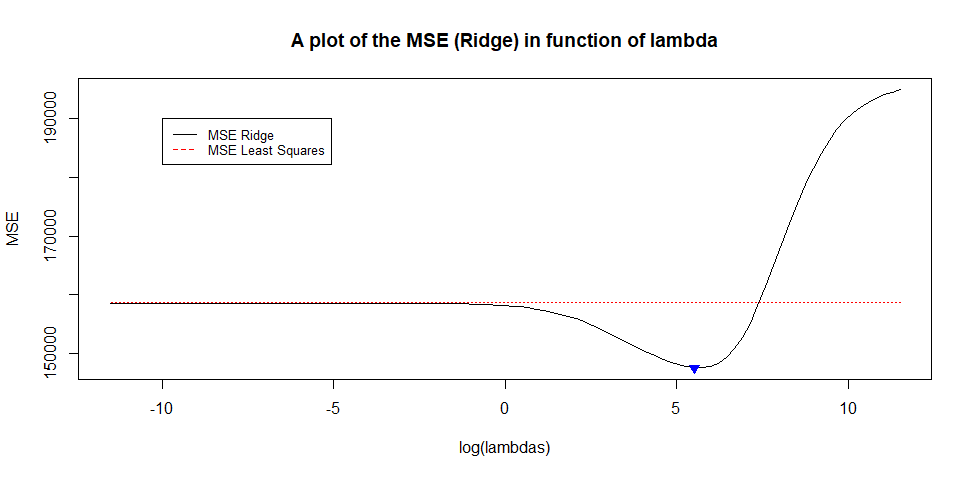
\includegraphics[width=\linewidth]{Figures/RidgeVSLSS.png}
    \caption{A plot of the mean squared error in function of $\lambda$. For reference, the mean squared error of the regular least squares fit is also plotted (red dashed line). The mean squared errors were calculated using Cross-Validation with training sets of size $100$.}
    \label{fig:RidgeVSLSS}
\end{figure}

\begin{figure}
    \centering
    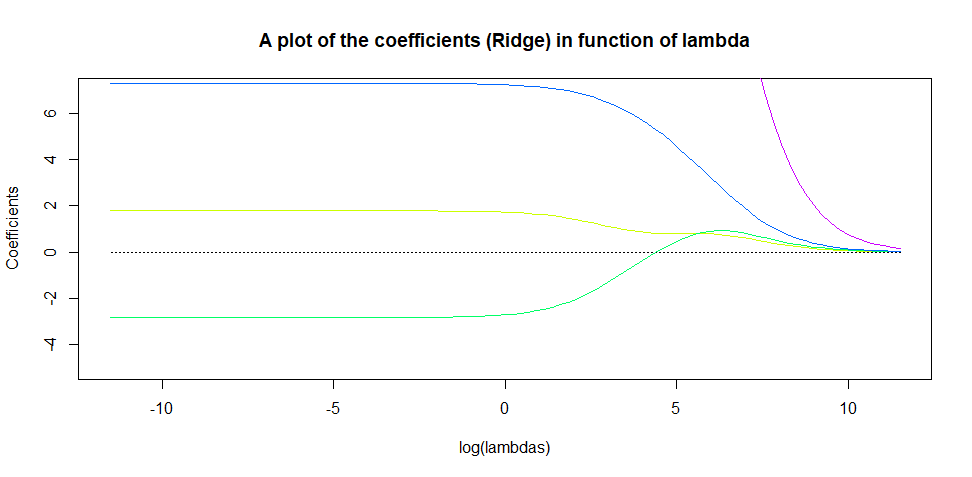
\includegraphics[width=\linewidth]{Figures/CoeffRidgeIFOLambda.png}
    \caption{The size of the regression coefficients plotted in function of $\lambda$.}
    \label{fig:CoeffRidge}
\end{figure}

% -------- A Historical Note ----------

\subsubsection{A Historical note}
The name \textit{ridge} regression was introduced by the inventors Art Hoerl and Bob Kennard. The method finds its origin as a solution to a multivariate optimization problem. The issue Hoerl and Kennard faced was that the optimal/maximal values of there optimization problem all laid on a line, which graphically looks like a ridge of a mountain, hence the name. This made the problem numerically hard to solve, so Hoerl and Kennard had to come up with a better method, which they called \textit{ridge analysis}. This method later found its way into statistics where it is known as \textit{ridge regression}.~\cite{Hoerl2020}

%---------------------------------------
%-------------- the Lasso --------------
%---------------------------------------

\subsection{The Lasso} \label{sec:Lasso}
In the previous section we attempted to solve the issue that regular regression has high variance when $n \approx p$. This led to what is known as ridge regression. There was, however, another problem with regular regression mentioned at the end of Section~\ref{sec:1.1.LR}, namely the issue of model interpretability. While ridge regression shrinks the coefficients towards zero, it does not set any of them equal to zero. The solution to this problem is subtle yet far reaching. It will appear that when we measure the size of the coefficients in $L_1$ norm, the least important coefficients will be set to zero.\\
\\
The Lasso\footnote{The term Lasso is an acronym for 'Least Absolute Shrinkage and Selection Operator'~\cite{Kas2018}} minimizes the following expression:
\begin{equation} \label{eq:Lasso}
    \begin{aligned}
        \hat{\beta}{}^{\text{lasso}} = \argmin_{\beta}\bigg\{\sum_{i=1}^N \bigg(y_i - \beta_0 - \sum_{j=1}^p x_{ij}\beta_j\bigg)^2\bigg\} \newline \text{, subject to } \sum_{i=1}^p |\beta_i| < t.
    \end{aligned}
\end{equation}
Or, equivalently,
\begin{equation}\label{eq:LassoAlt}
    \hat{\beta}{}^{\textrm{lasso}} = \argmin_{\beta}\bigg\{\sum_{i=1}^N \bigg(y_i - \beta_0 - \sum_{j=1}^p x_{ij}\beta_j\bigg)^2 + \lambda \sum_{i=1}^p |\beta_i|\bigg\}.
\end{equation}
Similar to ridge regression, the parameter $\lambda$ should be properly chosen by the statistician. We will explain how in Section~\ref{sec:4.CV&PS}.\\
\\
It is not immediately clear why the Lasso will make some regression coefficients exactly zero. A pictorial representation of the situation, given in Figures~\ref{fig:RidgeContour} and~\ref{fig:LassoContour}, will shed light on this phenomenon. This representation was heavily inspired on Figure 6.7 in \textit{Introduction to Statistical Learning}~\cite{ISL2013}. Figure~\ref{fig:RidgeContour} shows a geometric interpretation of equation~\eqref{eq:RidgeAlt}. We recall this equation below:
\begin{equation*}
    \begin{aligned}
        \hat{\beta}{}^{\text{ridge}} = \argmin_{\beta}\bigg\{\sum_{i=1}^N \bigg(y_i - \beta_0 - \sum_{j=1}^p x_{ij}\beta_j\bigg)^2\bigg\} \newline \text{, subject to } \sum_{i=1}^p \beta_i^2 < t
    \end{aligned}
\end{equation*}
This equation expresses that we want to find the point inside the open sphere $B(0,t)$, where we measure distance using the $L_2$-norm, that minimizes the residual sum of squares (RSS). If we plot the equicontours of the RSS, then the problem can be interpreted as finding the point of intersection of the equicontours with $B(0,t)$. The vector of coefficients obtained using regular regression is shown in the figure as $\hat{\beta}$. If we take $t$ large enough (which corresponds with taking $\lambda$ small enough, i.e. imposing only a small penalty on the size of the regression coefficients), then the blue region will contain $\hat{\beta}$ and the ridge regression coefficients will just be the regular regression coefficients. Building further on this idea we can see that if we set $\lambda = 0$, or equivalently $t = \infty$, ridge regression will always return the regular regression coefficients. This could also be easily seen directly from equation~\eqref{eq:RidgeAlt}.\\
\\
In a completely similar way we can make a geometric interpretation of equation~\eqref{eq:Lasso}. Not only does this aid in getting an intuitive understanding of what the Lasso does, it also shows why the Lasso puts some coefficients equal to zero. The reason for this is that open 'spheres' in $L_1$-norm are squares and thus have corners. Moreover, these corners are located on the axis, which are precisely the points in the coefficient space where some coefficients are equal to zero. It can be seen from Figure~\eqref{fig:LassoContour} that in many cases, the equicontours of the RSS will intersect the blue region in a corner if $\lambda$ is chosen small enough.\\
\\
The extra advantage that the Lasso has over ridge regression does come at a cost: It is more difficult to calculate. The reason for this is that in ridge regression, we want to minimize a quadratic expression with respect to a quadratic constraint. This makes the optimization problem a linear problem, and thus easy to solve. The optimization problem for the Lasso is non-linear due to the non-quadratic constraint. Luckily, there are efficient algorithms available for computing the Lasso just as fast as the ridge coefficients.

\begin{figure}[h!]
    \centering
    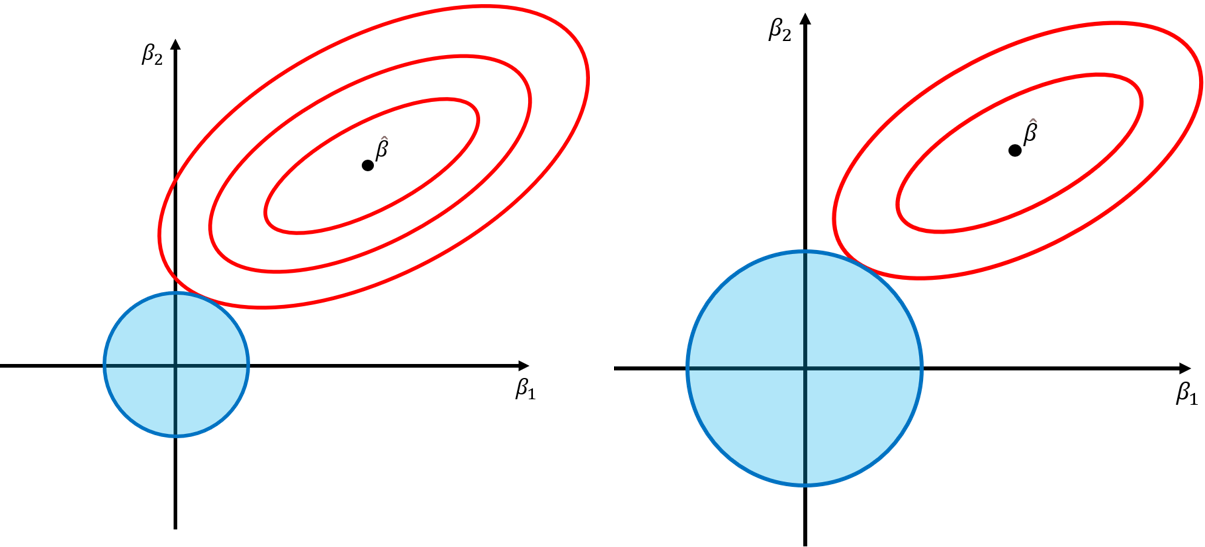
\includegraphics[width = \linewidth]{Figures/RidgeContour.png}
    \caption{The region $L_2(\beta) = \beta_1^2 + \beta_2^2 \leqslant t$ (blue) for two values of $t$ and the equicontours of the residual sum of squares. The point $\hat{\beta}$ represents the regular least squares regression coefficient vector.}
    \label{fig:RidgeContour}
    \vspace{10pt}
    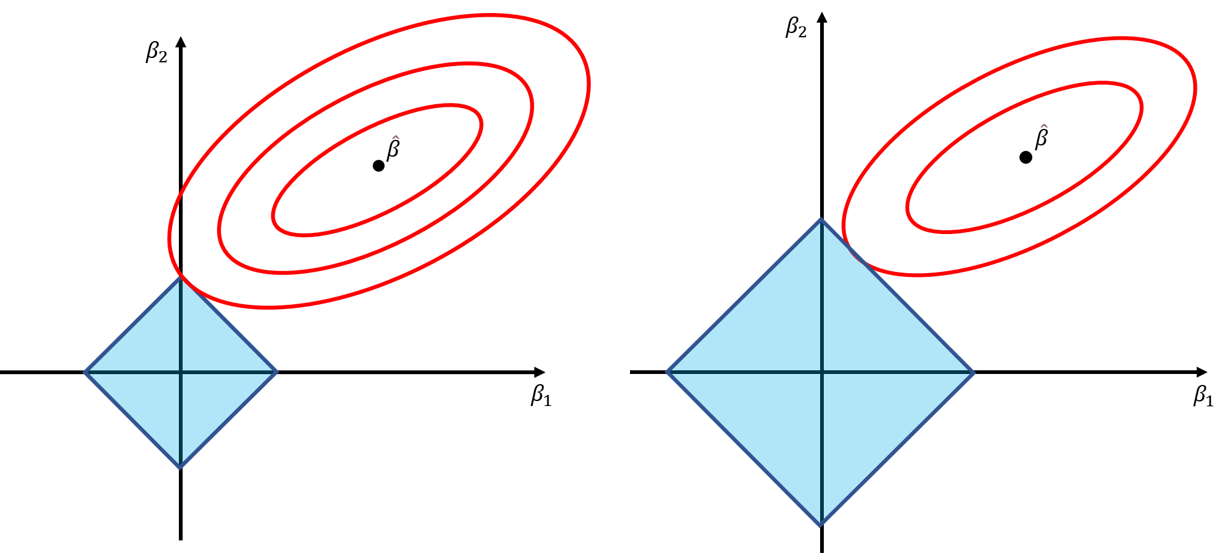
\includegraphics[width = \linewidth]{Figures/LassoContour.png}
    \caption{The region $L_1(\beta) = |\beta_1|+|\beta_2| \leqslant t$ (blue) for two values of $t$ and the equicontours of the residual sum of squares (red). If $t$ is taken small enough, the coefficient $\beta_2$ will be set equal to zero.}
    \label{fig:LassoContour}
\end{figure}

% ------ Comparison with regular regression ---------

\subsubsection{Comparison with regular regression}
In this small section we compare the Lasso to regular regression with an example in $R$ using the same data set as in Section~\ref{sec:PractRidgeComparison} (where we again restrict the data set in the same way). We use Cross-Validation to compute the prediction errors with training sets of size $100$.\\
\\
From Figure~\ref{fig:LassoVSLSS} it is clear that improvement upon the regular least squares fit is possible if we choose the correct value for $\lambda$, indicated by the blue triangle. Note that this is a different value then the one found in Section~\ref{sec:PractRidgeComparison}. As stated in that section, Lasso is a also a shrinkage methods. This is illustrated in Figure~\ref{fig:CoeffLasso}.

\begin{figure}
    \centering
    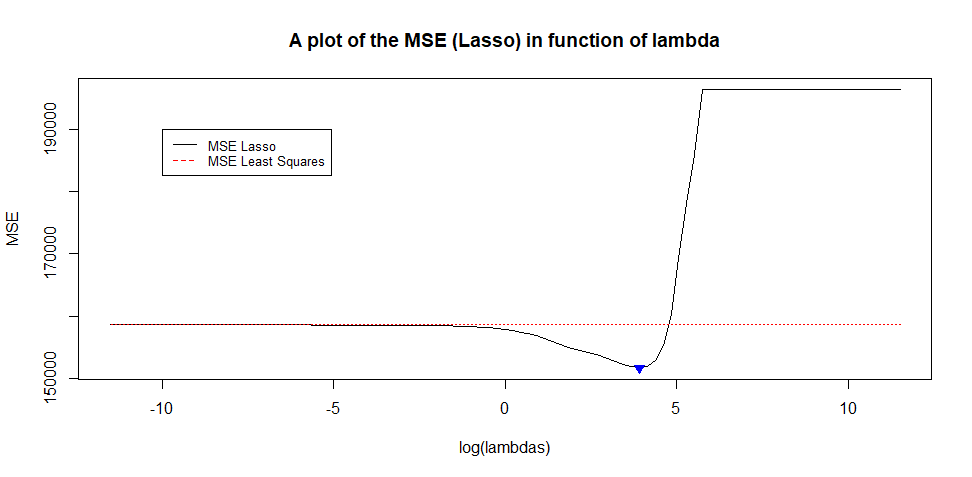
\includegraphics[width=\linewidth]{Figures/LASSOVSLSS.png}
    \caption{A plot of the mean squared error in function of $\lambda$. For reference, the mean squared error of the regular least squares fit is also plotted (red dashed line). The least squared errors were calculated using Cross-Validation with training sets of size $100$.}
    \label{fig:LassoVSLSS}
\end{figure}

\begin{figure}
    \centering
    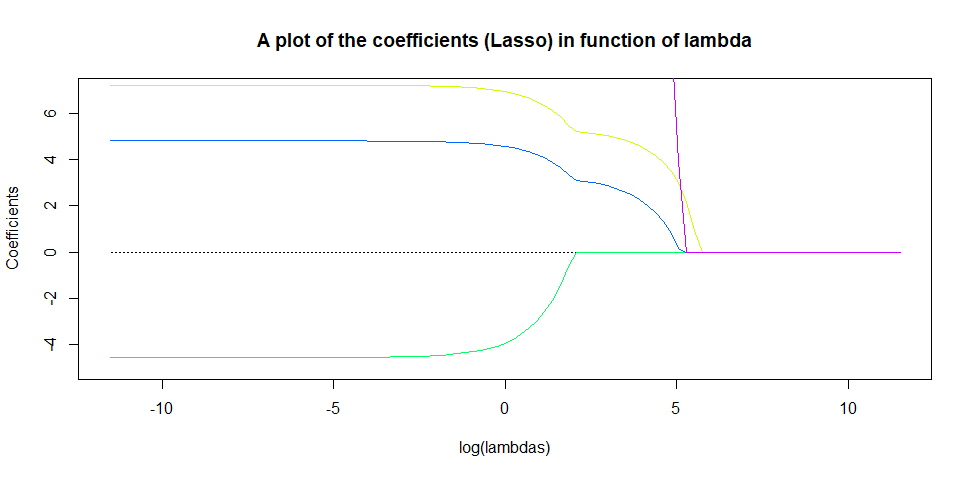
\includegraphics[width = \linewidth]{Figures/CoeffLASSOIFOLambda.png}
    \caption{The coefficients of the Lasso model in function of $\lambda$.}
    \label{fig:CoeffLasso}
\end{figure}

% --------------------------------------------------------
% ---------- Subset selection methods --------------------
% --------------------------------------------------------

\subsection{Subset selection methods}
We conclude this chapter by briefly discussing another approach to improve regular regression. We recall again the two main issues.
\begin{itemize}
    \item \textit{Prediction accuracy}: If $n \gg p$, then least squares fitting will have low variance. However, if $n$ is not much larger than $p$, least squares fitting tends to have high variance (overfitting). If $p > n$, then the variance is even infinite.
    \item \textit{Model interpretability}: Least squares fitting takes all predictors into account. This makes the model often difficult to interpret.
\end{itemize}
In Section~\ref{sec:RidgeRegression} we started by addressing the problem of \textit{prediction accuracy}, which led us to ridge regression. Section~\ref{sec:Lasso} then introduced the Lasso, which also took the issue of \textit{model interpretability} into account. Subset selection methods address the \textit{model interpretability} problem first. They select a subset of the parameters and then perform regular regression on this subset. The difficulty here is in selecting the best subset, that is, the subset for which the model will have the smallest variance.

\subsubsection{Best subset selection}
A naive algorithm to find the best subset is called \textit{Best Subset Selection}. Suppose we want to find the best subset of size $k \leqslant p$. To this end, we can construct all subsets of size $k$ from the set of predictors, calculate for each of these subsets the least squares regression fit and finally, pick the one with the smallest variance. While this is a feasible approach if the number of predictors is not too high $(p \leqslant 40)$\footnote{If $p = 40$ and $k = 20$, we would need to fit a least squares model $\binom{40}{20} \approx 1.4*10^{11}$ times.}, the method quickly becomes computationally too heavy if $p$ increases. Other methods, like \textit{Forward-} of \textit{Backward-stepwise selection} should be used. These methods do not guarantee to select the best subset but require much less computational effort. For further information, we refer to the literature~\cite{ESL2009}~\cite{ISL2013}.
\newpage
\section{Cross-Validation and parameter selection} \label{sec:4.CV&PS}

Cross-Validation can be used as a method of assessing the quality of a model, also known as \textit{Model assessment}. It can also be used to select the appropriate level of flexibility, also known as \textit{Model selection}. We will use Cross-Validation to select the tuning parameter $\lambda$ which minimizes the MSE. \\

In this section we will first show some methods of applying cross-validation and parameter tuning. Later, we will apply cross-validation to our models of the different types of regression we used in section~\ref{sec:3.PR}. We will then compare these types of regression in section~\ref{sec:4.CV&PS}. 

%--------------------------------------------
% --- Different types of Cross-Validation ---
%--------------------------------------------

\subsection{Different types of Cross-Validation}

% - K-fold Cross-Validation - 

\subsubsection{K-fold Cross-Validation}

% - Leave-one-out Cross-Validation (LOOCV) - 

\subsubsection{Leave-one-out Cross-Validation (LOOCV)}

%--------------------------------------------
% --- Applying 10-fold Cross-Validation ---
%--------------------------------------------

\subsection{Applying 10-fold Cross-Validation}

% - Linear regression - 

\subsubsection{Linear regression}

% - Ridge regression - 

\subsubsection{Ridge regression}

% - The Lasso - 

\subsubsection{The Lasso}
\newpage
\section{Comparison between the ridge and Lasso estimators} \label{sec:5.CRL}
We now have all the necessary tools to compare ridge regression with the Lasso. We do so with an elaborate example in R. The data set used in the rest of this section was found on \textit{Kaggle.com} \cite{EpiR}.

\subsection{The data}
The data set we will be using is about recipes from a popular website. It contains \num{20 025} observations (i.e. recipes) of \num{680} variables. Most of these variables are binary, indicating categories such as \textit{contains cucumber} or \textit{is a 22-minute meal}. Each recipe also has a \textit{rating}: a value that measures how well liked the recipe is by the users of the website.

In what follows, we will try to analyze the effect of all these variables on the rating of the recipes with regular least squares regression, ridge regression and the Lasso. We will compare their prediction accuracy and, along the way, illustrate some properties of the ridge and Lasso estimator. Lastly, we use the Lasso the find out which ingredients we should use and which styles of cooking we should follow in order to get the statistically most liked recipe.

Before we can begin, we must first remove all observations in the data set that contain values \textit{NA} as the built-in methods from the \textit{GLMNET}-package fail when these values are present. We also rename some badly named columns, remove the column containing the names of the recipes as this is not a predictor and restrict the data set to its first \num{15 000} observations. This last modification is done in order to work with nicely rounded numbers, which will be useful when dividing the observations into training and test sets, as well as reducing computation time. All of these modifications leave us with a data set containing 15 000 observations of 679 variables.

To illustrate the advantage of ridge and Lasso over regular least squares regression when $n \approx p$ we also simulate a small data set containing 120 observations of 51 variables (this way we have 50 predictors for the variable \textit{rating}). The reason why we simulate this data instead of just restricting the existing data set is that the latter leads to linearly dependent columns, so that we cannot apply linear regression.

\subsection{Regular least squares regression}
When we try to apply linear regression on the data set, the method fails. This failure is probably due to some columns of the data matrix being linearly dependent. Therefore other methods like ridge regression or the Lasso should be used. We also apply linear regression on the simulated data set. Since $n \approx p$, the MSE is very high, attaining a value of \num{24.3630}. This number means that, on average, the score we predict will be wrong by about $\sqrt{24.3630} \approx 5$ points. Since the scores is a number between $0$ and $5$, we get (almost) no valuable information from this model.

\subsection{Subset selection using the Lasso} \label{sec:SubsetSelectionUsingLasso}
Next we apply the Lasso to the data set and see which predictors it selects as the 10 most important. We get the following result:
\begin{center}
\begin{tabular}{ccc}
    \vspace{3pt}
     "caviar" & "cuba" & "dorie greenspan"\\
     \vspace{3pt}
     "germany" & "kitchen olympics" & "pancake"\\
     \vspace{3pt}
     "philippines" & "sardine" & "sorbet"\\
     & "leftovers" &
\end{tabular}
\end{center}
Note that these categories can either indicate a very high or very low rating.\\
\\
In order to test that the Lasso indeed indicates which predictors are the most important, we can artificially modify one predictor of the data set to be a 'perfect predictor' of the rating. In this example, we take the predictor \textit{22-minute meal} and set it to 1 if the rating of the recipe is bigger then 3. Therefore, the value of \textit{22-minute meal} should give a very good indication of the rating of the recipe and as a consequence, the Lasso should give it a high regression coefficient. Implementing the above into R and applying the Lasso, we get:
\begin{center}
    \begin{tabular}{ccc}
    \vspace{3pt}
        "22-minute meals" & "3-ingredient recipes" & "biscuit"\\
        \vspace{3pt}
        "flaming hot summer" & "gin" & "house \& garden"\\
        \vspace{3pt}
        "idaho" & "kansas" & "pastry"\\
        & "leftovers" &
    \end{tabular}
\end{center}
As expected, the Lasso now selects the predictor \textit{22-minute meal} as one of the 10 most important predictors.

Before continuing to the next section, we undo our changes to the variable \textit{22-minute meal}.

\subsection{Applying ridge regression} \label{sec:ApplyingRidgeRegression}
In this section we apply ridge regression on the data set. In order to properly asses the test error of the ridge model, we should carry out 10-fold Cross-Validation as explained in section~\ref{sec:4.CV&PS}. However, this would take hours of computing time. In order to have code that we -- or you, the reader -- can modify easily to explore the problem further without having to wait hours for the computations to complete each time, we opt to use training sets of size \num{10 000} and hence only have to compute the ridge model three times (even this already takes up a couple of minutes). Doing so gives us a test error of \num{1.5468}. Applying ridge regression on the simulated data set, we get a test error of \num{1.4888}. This is a tremendous improvement on the test error we got from the regular least squares model.

Like in Section~\ref{sec:PractRidgeComparison} we plot the size of the regression coefficients in function of $\lambda$ in Figure~\ref{fig:CoeffRidgeExample}. As this is only a general illustration of how the coefficients tend to evolve in function of $\lambda$, we part with Cross-Validation all together and just use a fixed training and test set. Figure~\ref{fig:CoeffRidgeExample} illustrates nicely how all coefficients get shrunk towards zero.

\begin{figure}
    \centering
    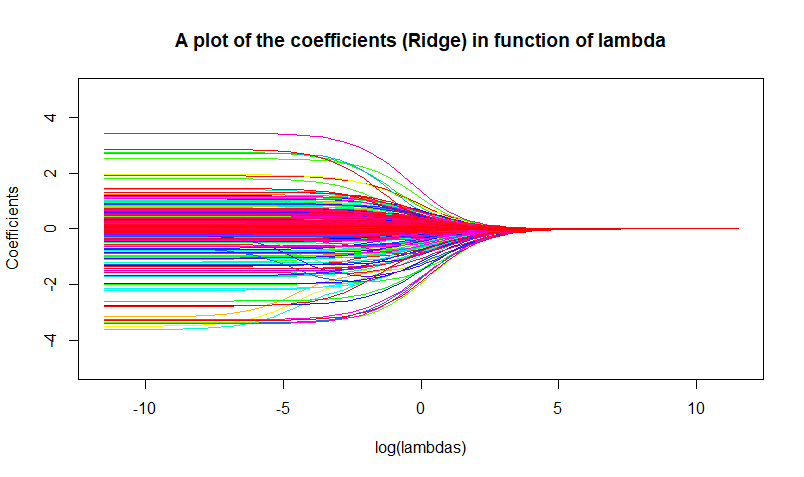
\includegraphics[width=\linewidth]{Figures/Coeff_Lambda_plot_ridge.png}
    \caption{The coefficients of the ridge model in function of $\lambda$.}
    \label{fig:CoeffRidgeExample}
\end{figure}

\subsection{Applying the Lasso} \label{sec:ApplyingTheLasso}
We continue our analysis by applying the Lasso on the data set. For similar reasons as in Section~\ref{sec:ApplyingRidgeRegression} we use training sets of size \num{10 000} and thus compute the Lasso model only thrice. The resulting test error of the model is \num{1.1790}. This is better than that of the ridge model. Applying the Lasso on the simulated data set, we get a test error of \num{1.4879}. This is also better than the one we got using ridge regression, although only very slightly. A plot of the coefficients of the Lasso model is given in Figure~\ref{fig:CoeffLassoExample}.

\begin{figure}
    \centering
    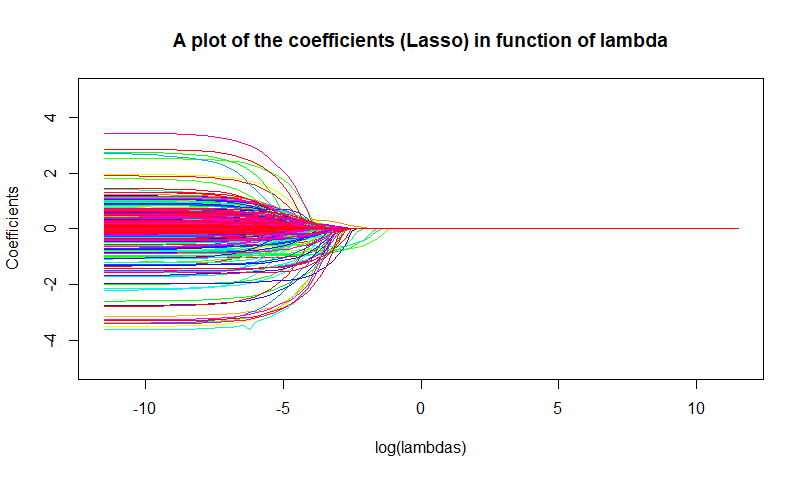
\includegraphics[width=\linewidth]{Figures/Coeff_Lambda_plot_Lasso.png}
    \caption{The coefficients of the Lasso model in function of $\lambda$.}
    \label{fig:CoeffLassoExample}
\end{figure}

Figure~\ref{fig:Comparison_ridge_Lasso} compares, for fixed training and test set, the MSE of the ridge and Lasso model.\footnote{Hence we again do not implement any form of Cross-Validation for this figure. this is why the mean squared errors for the optimal values of lambda slightly differ from the mean squared errors we got in Section~\ref{sec:ApplyingRidgeRegression} and~\ref{sec:ApplyingTheLasso}.} The plot shows an important difference in characteristic of ridge and Lasso estimation: The curve of the mean squared error appears smooth for ridge regression, but shows a discontinuity in the first derivative in the case of the Lasso. This difference can be explained by the 'subset-selection property' of the latter estimator. When regression coefficients for the Lasso model get small enough, they get set exactly equal to zero and remain zero, in contrast to ridge regression, where they \textit{approach} zero and can oscillate around zero. A similar difference in behaviour can also be seen from Figures~\ref{fig:CoeffRidge} and~\ref{fig:CoeffLasso}.

\begin{figure}
    \centering
    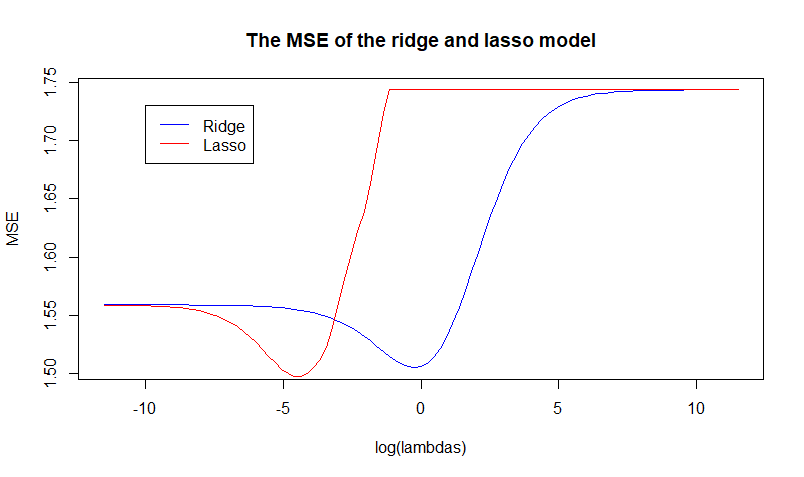
\includegraphics[width=\linewidth]{Figures/Comparison_ridge_lasso.png}
    \caption{A plot comparing the MSE of the ridge and lasso model in function of $\lambda$. The models were computed with the same training data and the test errors were calculated with the same test data.}
    \label{fig:Comparison_ridge_Lasso}
\end{figure}

\subsection{Some data analysis using the Lasso}
To conclude this section, we perform some data analysis using the Lasso. More specifically, we try to answer the following two questions:
\begin{itemize}
    \item Which nutritional values \textit{calories}, \textit{fat}, \textit{protein} and \textit{sodium} should a recipe have to get the highest rating?
    \item What categories should a recipe belong to (or definitely not belong to) in order to have the highest rating?
\end{itemize}
To answer the first question, we restrict our data to just the 5 columns \textit{rating}, \textit{calories}, \textit{fat}, \textit{protein} and \textit{sodium} and apply the Lasso. We get the following output, listed in Table~\ref{tab:NutritionalValues}.
\begin{table}[h]
    \centering
    \begin{tabular}{cc}
         calories & \num{2.258779e-08}\\
         protein & \num{5.776022e-06}\\
         fat & \num{-7.529660e-07}\\
         sodium & .
    \end{tabular}
    \caption{Analysis of the nutritional values}
    \label{tab:NutritionalValues}
\end{table}
From the regression coefficients we can see that recipes with high protein tend to get given a high rating, and that the amount of fat in a recipe has a negative impact on the rating. In other words: If we want a recipe with high rating, we should cook healthy!\\
\\
To answer the second question we perform the Lasso on the data set where the columns containing nutritional value (\textit{calories}, \textit{fat}, \textit{protein} and \textit{sodium}) have been removed. Similar to Section~\ref{sec:SubsetSelectionUsingLasso} we select the \num{10} predictors that have the highest coefficients in absolute value. This time we also note down their numerical values. The results are listed in Table~\ref{tab:Ingredients}.
\begin{table}[h]
    \centering
    \begin{tabular}{c|c}
        leftovers &  -3.45301190707604 \\
        kitchen olympics &  -2.68671340475449 \\
        germany &  -2.68045838198475 \\
        sardine &  -2.49597552609873 \\
        dorie greenspan &  -2.38525177319951 \\
        caviar &  -2.24005956660075 \\
        cuba &  -2.11104676712887 \\
        philippines &  -2.09261833766479 \\
        pancake &  -2.04455056659949 \\
        sorbet &  -1.87835922993761 \\
    \end{tabular}
    \caption{Analysis of the different categories}
    \label{tab:Ingredients}
\end{table}
All of the categories above have a negative regression coefficient. This means we should definitely avoid designing a recipe that belongs to any of them. 
\newpage
\section{Conclusion}
\newpage
\section*{Questions}
\begin{itemize}
    \item Should the abstract come before or after the table of contents?
    \item How should we structure the paper? Is it ok as it is now or should we move Sections 2 and 3 into the introduction?
    \item Using the function \textit{G,LMnet} in R, the intercept changes as $\lambda$ is varied. Why is this the case? The calculation of the intercept in the books is done by $\frac{1}{N}\sum_{i=1}^N y_i$, which is independent of $\lambda$.
    \item What is the $R^2$ test statistic and where is it used?
    \item Is this source~\cite{Kj2018} okay? --> find book
\end{itemize}

\section*{Structure of the paper}
\begin{enumerate}
    \item Abstract
    \item Introduction (Ilias)
    \item Penalized Regression (Ilias)
    \begin{enumerate}
        \item Motivation for penalized regression: Find a data set where normal regression fails ($n \approx p$ or even $n < p$).
        \item Introduce Ridge regression, explain and apply to data set
        \item Introduce Lasso, explain and apply to (preferably the same) data set
        \item Possibly explain some other methods (like subset selection)
    \end{enumerate}
    \item Cross-validation and parameter selection (Nina)
    \begin{enumerate}
        \item Motivate importance of parameter selection and need for method of comparing different parameters
        \item Introduce cross-validation
    \end{enumerate}
    \item Comparison of Ridge and Lasso --> adhv epicurious dataset.
    \begin{enumerate}
        \item 700 predictors is not easy to interpret. Running Lasso on the data set will eliminate a lot of variables.
        \item Set the tag for '$22$-minute meals' of all dished that have high rating to $1$ and run Lasso. It should select that predictor.
        \item Restricting the data set to its first 700 rows makes $n \approx p$. Running Ridge on the data set will (hopefully) give better test errors than regular regression
        \item Which regression methods has the lowest test error? 
        \item Possibility to test multiple types of CV (although $k$-fold CV is best so maybe just use that?)
        \item Fun questions:
        \begin{itemize}
            \item What ingredients should we mix to get the highest rating?
            \item What are the proportions of nutritional values that get would get us the highest rating?
        \end{itemize}
    \end{enumerate}
    \item Conclusion (Nina)
    \begin{itemize}
        \item Write something about SCAD?
        \item Write something about LAR?
        \item Write something about where this is used?
        \item Summarize our findings?
        \item Compare our own implementation of Ridge and Lasso to the one in the R-package?
    \end{itemize}
\end{enumerate}

\section*{Summary}
A great summary of ridge regression and lasso, as well as some implementation tips, can be found on the website given in \cite{Kas2018}. A Notebook going through Lab 2 of ISLR can be found in the website given in the footnote\footnote{http://www.science.smith.edu/~jcrouser/SDS293/labs/lab10-r.html}\\
\\
In this chapter we summarize for our-self what we are eventually going to write about in the paper.

\subsection*{The Elements of Statistical Learning}
All of the information below came from the book "Elements of Statistical Learning", unless stated otherwise.

\subsubsection*{Introduction}
Learning problems
\begin{itemize}
    \item Supervised learning: predict the value of an outcome measure based on a number of input measures (f.e. regression).
    \item Unsupervised learning: No outcome measure, goal is to describe the associations and patterns in input measures (f.e. classification).
\end{itemize}

\subsubsection*{Chapter 3: Linear methods for regression}
Linear regression
\begin{itemize}
    \item Given is a data matrix containing $N$ data vectors $x_i \in \mathbb{R}^p$ \begin{equation*}
        \textbf{X} = \begin{pmatrix}
        1 & x_{11} & x_{12} & \dots & x_{1p}\\
        1 & x_{21} & x_{22} & \dots & x_{2p}\\
        \vdots & \vdots & \vdots & \ddots & \vdots\\
        1 & x_{N1} & x_{N2} & \dots & x_{Np}
        \end{pmatrix}
    \end{equation*}
    where we assume that its column space has full rank.
    \item We want to minimize the Residual Sum of Squares: \begin{equation*}
        \text{RSS}(\beta) = (\textbf{y} - \textbf{X}\beta)^T(\textbf{y} - \textbf{X}\beta).
    \end{equation*}
    \item This is achieved for $\beta = (\textbf{X}^T\textbf{X})^{-1}\textbf{X}^T\textbf{y}$.
    \item We denote the predicted values as $\hat{y}$ and calculate them as \begin{equation*}
        \hat{y} = \textbf{X}\beta = \textbf{X}(\textbf{X}^T\textbf{X})^{-1}\textbf{X}^T\textbf{y} = \textbf{H}y.
    \end{equation*}
    The matrix $\textbf{H}$ is often called the \textit{hat} matrix as it \textit{puts the hat on the vector \textbf{y}}. It projects the vector $\textbf{y}$ orthogonally onto the column space of \textbf{X}.
    \item Gauss-Markov theorem: The least squares estimator of $\beta$ is the one with the smallest variance among all linear unbiased estimators of $\beta$. There could, however, exist biased estimators with smaller mean squared error (= variance).
\end{itemize}
An example of linear regression (on prostate cancer) starts on p. 49. This example will return later in the section about the $LASSO$-estimator.\\
\\
Chapter 3.2.3: "Multiple regression from simple univariate regression" is pretty vague, I don't understand it. \\
\\
Problems with least squares estimates:
\begin{itemize}
    \item Prediction accuracy: Least squares estimates have low bias but large variance. Sacrificing a little bit of bias to reduce variance might improve the overall accuracy.
    \item Least squares estimates take all variables into account. For the sake of easy to interpret models, it is sometimes advisable to reduce the number of variables (and therefor sacrificing some bias) to better understand "the big picture" (i.e. see what variables matter the most when trying to predict certain outcomes).
\end{itemize}
This brings us to subset selection.
\begin{itemize}
    \item Subset selection looks to retain only a subset of the variables and eliminate the rest from the model.
    \item \textit{Best-subset selection}: Finds for each $k$ the subset of size $k$ that gives the smallest residual sum of squares. The higher $k$, the lower $RSS$, but the more complex the model becomes.
    \item \textit{Forward-stepwise selection}: Starts with the intercept and sequentially adds predictors that most improve the fit.
    \item \textit{Backward-stepwise selection}: Starts with the full model and sequentially deletes predictors that have the least impact on the fit.
    \item \textit{Forward-stagewise regression}: (probably) not important for our topic.
\end{itemize}
\underline{\textbf{3.4:} Shrinkage methods}\\
Often times subset selection is too 'crude' of a method to reduce the prediction error of the full model as it is a discrete method: It either retains or discards a predictor. Shrinkage methods are more continuous and don't suffer as much from high variability. 

\begin{itemize}

    % The ridge estimator
    \item \textit{Ridge regression}: Ridge regression shrinks the regression coefficients by imposing a penalty on their size. Unlike normal linear regression, where one tries to minimize the Residual Sum of Squares \begin{equation*}
        \text{RSS}(\beta) = \argmin_{\beta}\bigg\{\sum_{i=1}^N \bigg( y_i - \beta_0 - \sum_{j=1}^p x_{ij}\beta_j\bigg)^2\bigg\}
    \end{equation*}
    we minimize the following expression \begin{equation}\label{eq:ridgeEstimator}
        \hat{\beta}{}^{\text{ridge}} = \argmin_{\beta}\bigg\{\sum_{i=1}^N \bigg( y_i - \beta_0 - \sum_{j=1}^p x_{ij}\beta_j\bigg)^2 + \lambda \sum_{i=1}^p \beta_i^2\bigg\}
    \end{equation}
    where $\lambda$ is the complexity parameter, it controls how much the coefficients are shrunk. Equivalently, we can write equation \eqref{eq:ridgeEstimator} as \begin{equation}\label{eq:ridgeEstimatorEquivalent}
    \begin{aligned}
        \hat{\beta}{}^{\text{ridge}} = \argmin_{\beta}\bigg\{\sum_{i=1}^N \bigg(y_i - \beta_0 - \sum_{j=1}^p x_{ij}\beta_j\bigg)^2\bigg\} \newline \text{, subject to } \sum_{i=1}^p \beta_i^2 < t
    \end{aligned}
    \end{equation}
    which explicitly states the size constraint on the parameters. Ridge regression is to be preferred over normal regression when there are many correlated variables in the model, as that can lead to variables getting very large positive and negative coefficients that ultimately cancel each other out (say for example $y = 10^{16}x_1 - 5*10^{15}x_2$). By imposing a size constraint on the parameters, this problem is alleviated.\\
    \\
    \textbf{(For question 2)} Also notice that the intercept coefficient $\beta_0$ has been left out of the penalization. Penalization of the intercept would make the procedure depend on the origin chosen for $Y$, that is, say we shift $Y$ in some direction by adding a constant $c$ to its components, then this would not simply result in a shift of the predictions by the same amount $c$.\\
    \\
    Writing equation \eqref{eq:ridgeEstimator} in matrix notation (after centralizing the data and setting $\beta_0 = \frac{1}{N} \sum_{i=1}^N y_i$) with $\beta = (\beta_1, \dots \beta_p)$, we get
    \begin{equation}\label{RidgeMatrixNotation}
        RSS(\lambda) = (\textbf{y} - \textbf{X}\beta)^T(\textbf{y} - \textbf{X}\beta) + \lambda\beta^T\beta
    \end{equation}
    The solution to this minimization problem can be seen to be
    \begin{equation}
        \hat{\beta}{}^{\textrm{ridge}} = (\textbf{X}^T\textbf{X} + \lambda\textbf{I})^{-1}\textbf{X}^T\textbf{y}.
    \end{equation}
    We define the \textit{effective degrees of freedom} of the ridge regression fit to be \begin{align*}
        \textrm{df}(\lambda) & = \textrm{tr}[\textbf{X}(\textbf{X}^T\textbf{X} + \lambda\textbf{I})^{-1}\textbf{X}^T]\\
        & = \sum_{i=1}^p \frac{d_j^2}{d_j^2 + \lambda}
    \end{align*}
    The coefficients $d_j$ come from the singular value decomposition (SVD) of the data-matrix \textbf{X} \begin{equation*}
        \textbf{X} = \textbf{UDV}^T.
    \end{equation*}
    Here $\textbf{U} \in \mathbb{R}^{N \times p}$, $\textbf{D} \in \mathbb{R}^{p \times p}$ and $\textbf{V} \in \mathbb{R}^{p \times p}$. The matrices \textbf{U} and \textbf{V} are orthonormal matrices and the matrix \textbf{D} is a diagonal matrix containing the singular values $d_j$ with $d_1 \geqslant d_2 \geqslant \dots \geqslant d_p$ of \textbf{X}.\\
    \\
    Substituting \textbf{X} with its SVD in the formula for the regular regression coefficients, we obtain
    \begin{align*}
        \textbf{X}\beta &  = \textbf{X}(\textbf{X}^T\textbf{X})^{-1}\textbf{X}^T\textbf{y}\\
        & = \textbf{U}\textbf{U}^T\textbf{y}.
    \end{align*}
    It can be shown that $\textbf{U}\textbf{U}^T = \textbf{H}$ is the orthogonal projector onto the column space of \textbf{X}. Doing the same for the ridge estimator $\hat{\beta}{}^{\textrm{ridge}}$ we obtain
    \begin{align*}
        \textbf{X}\hat{\beta}{}^{\textrm{ridge}} & = \textbf{X}(\textbf{X}^T\textbf{X} + \lambda\textbf{I})^{-1}\textbf{X}^T\textbf{y}\\
        & = \sum_{j=1}^p \textbf{u}_j\frac{d_j^2}{d_j^2 + \lambda}\textbf{u}_j^T\textbf{y}
    \end{align*}
    We see that, like linear regression, ridge regression computes the coordinated of \textbf{y} with respect to the orthonormal basis \textbf{U}. It then shrinks these coordinates with the factor $\frac{d_j^2}{d_j^2 + \lambda}$. This means that a greater amount of shrinkage is applied to the coordinates of basis vectors that correspond to smaller $d_j$'s. It can be shown that the values $d_j$ also correspond to the principal components of \textbf{X} (see book p. 66). The smallest principle component $d_p$ is the one that explains the least amount of variance of the model and gets shrunk the most.
    
    % The lasso estimator
    \item \textit{The Lasso}: Very similar to ridge regression, the lasso\footnote{Least Absolute Shrinkage and Selection Operator, \cite{Kas2018}} is also a shrinkage method but there is a subtle yet important difference. The lasso estimate is defined by \begin{equation}\label{eq:lassoEstimate}
        \hat{\beta}{}^{\textrm{lasso}} = \argmin_{\beta}\bigg\{\frac{1}{2}\sum_{i=1}^N \bigg(y_i - \beta_0 - \sum_{j=1}^p x_{ij}\beta_j\bigg)^2 + \lambda \sum_{i=1}^p |\beta_i|\bigg\}
    \end{equation}
    or equivalently,
    \begin{equation*}
        \begin{aligned}
        \hat{\beta}{}^{\text{lasso}} = \argmin_{\beta}\bigg\{\sum_{i=1}^N \bigg(y_i - \beta_0 - \sum_{j=1}^p x_{ij}\beta_j\bigg)^2\bigg\} \newline \text{, subject to } \sum_{i=1}^p |\beta_i| < t.
    \end{aligned}
    \end{equation*}
    As can be seen from the definitions, the ridge and lasso estimates only differ in how they measure the size of the regression coefficients $\beta$. The ridge estimate measures $\beta$ in $L_2$ norm (also known as Euclidean distance) while the lasso estimate measures $\beta$ in $L_1$ norm (which is also known as Manhattan or Taxicab distance)\footnote{The existence of the ridge and lasso estimate could imply the existence of a whole class of estimates similar to ridge and lasso, but differing in what norm $L_p$ they use to measure the size of $\beta$. This is indeed the case: this class of estimators is known as the Bridge estimators \cite{WWM2020}. It is even possible to let $p$ take on non-integer values. If we set $p=0$, the method corresponds to variable subset selection as the penalty simply counts the number of non-zero parameters.}.
\end{itemize}

\underline{\textbf{3.4.3:} A comparison between subset selection, ridge estimates and lasso estimates.}
\begin{itemize}
    \item subset-selection: hard thresholding $\rightarrow$ A predictor is either included or excluded.
    \item ridge and lasso estimates: soft thresholding $\rightarrow$ Shrinkage of coefficients.
\end{itemize}
Both the ridge and lasso methods can be visualized by figure~\ref{fig:Fig3.11}.
\begin{figure}[h!]
    \centering
    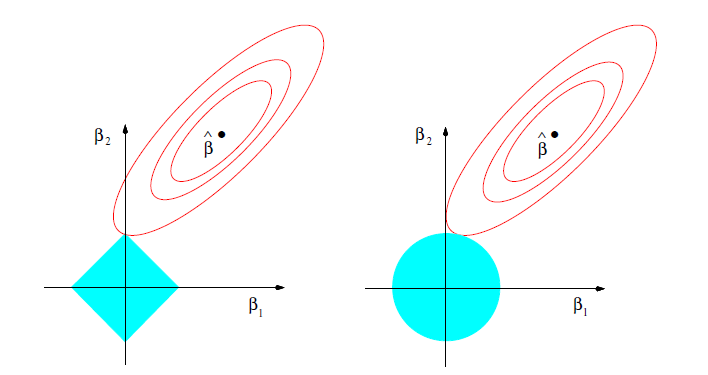
\includegraphics[width=\linewidth]{Figures/Figure3.11.PNG}
    \caption{Figure 3.11 from the book}
    \label{fig:Fig3.11}
\end{figure}
The methods find the first intersection of the region $L_p(\beta) < t$ and the elliptical contours of the residual sum of squares. The region $L_p(\beta) < t$ is a circle of if $p=2$ and diamond-shaped if $p=1$. Ideally, we would like the intersection to be at a point where (many) $\beta_j$'s are zero, so we can simplify the model. Different elements of the bridge estimator class give rise to different blue regions.\\
\\
\underline{Eigen hersenspinsel, niet te veel aandacht aan besteden.}\\
A possibly interesting case is $p=0$, then the region is defined as $\{(x,y) \hspace{3pt} | \hspace{3pt} x^0 + y^0 = t\}$. The only possible value $t$ can take in this case is $1$ or $2$, corresponding to the the $x$-and $y$-axis, respectively the whole plain where we defined $0^0=0$.\\
\\
As a side note, the lasso, ridge regression and best subset selection can all be viewed as Bayes estimators of the correct prior distributions. Lastly, it is also possible to combine estimators. An example of this is the estimator introduced by Zou and Hastie (2005), which uses the \textit{Elastic-net} penalty \begin{equation*}
    \lambda\sum_{j=1}^p (\alpha\beta_j^2+(1-\alpha)|\beta_j|).
\end{equation*} It combines aspects from both ridge and lasso estimates and can be advantages in certain situations (especially computationally).\\
\\
\underline{\textbf{3.4.4:} Least Angle Regression (LAR)}
\begin{enumerate}
    \item Identify the predictor $x_i$ that is most correlated with the response.
    \item Move the coefficient $\beta_i^{\textrm{LAR}}$ of this predictor continuously towards its least squares coefficient $\beta_i^{\textrm{ls}}$, causing its correlation with the residual to decrease. In other words: try to find the variable that explains the most variance of the complete model en include it more and more into the new model.
    \item As soon as an other predictor $x_j$ "catches up" in terms of correlation with the residual, $x_j$ joins the active set and their coefficients are moved together towards their full least squares coefficients in such a way that the correlation of $x_i$ and $x_j$ with the response stays equal. This process ends at the full least squares fit.
\end{enumerate}
See also Algorithm 3.2 in the book on page 74.\\
\\
It can be shown that by a simple modification of this algorithm, an algorithm for the lasso estimate can be achieved (Algorithm 3.2a, page 76).\\
\\
Section 3.8 expands further on Lasso.

% ------------------------------------------------------------
% ----- Introduction to Statistical Learning: Chapter 5 ------
% ------------------------------------------------------------

\subsection*{Introduction to Statistical Learning (Chapter 5: Resampling methods)}
The aim of this section is to compile some important elements surrounding (cross-)validation. All of the information below came from the book "Introduction to Statistical Learning", unless stated otherwise.

\underline{Introduction}
\begin{itemize}
    \item Cross-validation can be used to estimate the test error associated with a given statistical learning method in order to evaluate its performance (also known as \textit{Model assessment}.
    \item Cross-validation can also be used to select the appropriate level of flexibility (also known as \textit{Model selection}.
\end{itemize}

\underline{Cross-validation}
\begin{itemize}
    \item Problem: How to test whether a statistical model is a good model? Solutions: \begin{itemize}
        \item Use a test set (a set of data that is not used in the deriving of the model) to check whether the predictions match the data.\\
        \textbf{Problem:} Such a set is often not available.
        \item Use training data to check whether the predictions match the data. \\
        \textbf{Problem:} Such a test often grossly underestimates the true \textit{test error}.
        \item Make some perturbations on the training data and calculate the expected result. Then check whether the model predicts this expected result.
        \item Hold out a subset of the training data and test the derived model with this subset. It is this type of testing we're interested in.
    \end{itemize}
\end{itemize}

\underline{Validation set approach}
\begin{itemize}
    \item Randomly divide the observations into a \textit{training set} and a \textit{test set}. Derive a model based on the training set data.
    \item The validation set test error provides an estimate for the test error of the model (often measured in MSE).
    \item Problems: \begin{itemize}
        \item Since not all available data is used in the models (some of it is used to test the model), it can be expected that the estimated test error is higher than the test error that one would get when deriving the model based on all available data.
        \item Since we randomly divide the observations into two sets, there is a variability in the estimated test error. This variability tends to be quite high.
    \end{itemize}
\end{itemize}

\underline{Leave-On-Out Cross-validation (LOOCV)}
\begin{itemize}
    \item Apply the \textit{Validation set approach} as described above with a test set containing precisely one observation and the training set the other $n-1$ observations. Derive the model with the training set data and calculate the test error of the single test set element, call it $MSE_1$. Repeat this procedure $n$ times, one time for each element $y_i$ in the training set, with $\{y_i\}$ the test set. An estimation for the test error is then \begin{equation*}
        CV_{(n)} = \frac{1}{n}\sum_{i=1}^n MSE_i.
    \end{equation*}
    \item Tends to be computationally expensive as $n$ gets large.
    \item A nice shortcut exists in the case of least squares linear or polynomial regression. see page $180$.
\end{itemize}

\underline{K-fold Cross-Validation}
\begin{itemize}
    \item The observations are split into $k$ subsets of approximately equal size (also called \textit{folds}). The first fold is treated as the validation set, the other $k-1$ folds are used together as the training set. We then calculate the test error $MSE_1$ with the validation set. This process is repeated $k$ times, where each time we use a different fold as the validation set. An estimate for the test error is then \begin{equation*}
        CV_(k) = \frac{1}{k}\sum_{i=1}^k MSE_i
    \end{equation*}
    \item It is clear that LOOCV is a special case of $K$-fold CV. General $K$-fold CV has obvious computational advantages over LOOCV.
    \item In general, $5$- or $10$-fold Cross-validation is a more accurate test error estimation method than LOOCV. This might be surprising at first: Since we use more of the available data in LOOCV, we should expect LOOCV the be more accurate. While it is true that the bias of LOOCV is lower than, say, $10$-fold Cross-validation (for the model tested in LOOCV is nearly the model when using all available data, unlike the model tested in $10$-fold Cross-validation), it does not tell the whole story, variance must also be taken into account. Since the training data in LOOCV for each model is nearly identical, the test error estimates are going to be very correlated, leading to a high test error variance\footnote{A small change in one test error will imply nearly the same change in all other test errors because they are very correlated. Thus, the average of all test errors will have high variability.}. In the case of $10$-fold Cross-validation, this correlation will be much less, leading to a lower test error variance. The slight increase in bias is thus well made up for by the big decrease in variance, to such an extend that $10$-fold Cross-validation is better than LOOCV. (\textit{bias-variance trade-off})
\end{itemize}

% ------------------------------------------------------------
% ----- Introduction to Statistical Learning: Chapter 6 ------
% ------------------------------------------------------------

\subsection*{Introduction to Statistical Learning (Chapter 6: Linear model selection and Regularization)}
All of the information below came from the book "Introduction to Statistical Learning", unless stated otherwise.

\subsubsection*{Important notions}
In this subsection we list some important notions to understand what is written below.
\begin{itemize}
    \item Training error: The error (measured in RSS, $R^2$, \dots) of the training data with respect to the predicted values.
    \item Test error: The error (measured in RSS, $R^2$, \dots) of the test data with respect to their predicted values. Notice the important difference with training error: the parameters of the model were chosen based to best fit the training data, hence the training error will be as low as possible. The data from the test error, however, has had no influence on the model and is thus a better measure of 'how good' the model is.
    \item Null model: a model that contains no predictors.
    \item Cross-validation: Use test data to asses how good the model is (measure what the prediction error is). See also previous chapter.
    \item We say that \textit{a model has high variance} if a small change in training data leads to substantial changes in the coefficients $\beta$.
    \item Sparse model: models that involve only a subset of the variables.
\end{itemize}

\subsubsection*{Introduction}
Why do we want alternative procedures for least squares fitting?
\begin{itemize}
    \item \textit{Prediction accuracy}: If $n >> p$, then least squares fitting will have low variance. However, if $n$ is not much larger than $p$, least squares fitting tends to have high variance (overfitting). If $p > n$, then the variance is even infinite. By constraining or shrinking the estimated coefficients, we can lower the variance substantially at the cost of a minor increase in bias.
    \item \textit{Model interpretability}: Removing unnecessary variables improves the interpretablility of the result.
\end{itemize}

\subsubsection*{Subset selection}
\underline{Best subset selection}
\begin{itemize}
    \item Consider all subsets of $k$ predictors from the full model (with $n$ predictors). Calculate for each the least squares regression fit and pick the one with the lowest \textit{test error}.
    \item This method is computationally heavy and becomes unfeasible if $n > 40$.
\end{itemize}

\underline{Forward stepwise selection}
\begin{itemize}
    \item Algorithm: 
        \begin{enumerate}
        \item Start from the null model $\mathcal{M}_0$.
        \item Add the predictor that augments the current model the most. That is, find the predictor $x_{k+1}$ such that $\mathcal{M}_{k} \cup x_{k+1}$ has the lowest RSS. In this way, one achieves a sequence of models $\mathcal{M}_0, \mathcal{M}_1, \dots, \mathcal{M}_p$.
        \item Use cross-validation to select the best model in the above sequence. 
        \end{enumerate}
    \item This method is not guaranteed to find the best subset. 
\end{itemize}

\underline{Backwards stepwise selection}
\begin{itemize}
    \item Same as Forward stepwise selection, but instead of starting with a null model and sequentially adding predictors, we start with the full model and sequentially remove predictors.
    \item This method is not guaranteed to find the best subset.
\end{itemize}

\underline{Hybrid models}
Like Forward stepwise selection, but now at each step it is checked if a variable in the model is no longer useful so that it can be removed. This method tries to mimic better best subset selection.

\underline{Choosing the optimal model: What statistic to use?}
Section 6.1.3 in the book (p. 210). Could be useful.

\subsubsection*{Shrinkage methods}
Instead of using subsets, we use all $p$ predictors but restrain the coefficient estimates. This significantly reduces the variance of the model.\\
\\
\underline{Ridge regression}
\begin{itemize}
    \item Instead of minimizing the Residual Sum of Squared \begin{equation*}
        RSS = \sum_{i=1}^n \bigg( y_i - \beta_0 - \sum_{j=1}^p x_{ij}\beta_j\bigg)^2,
    \end{equation*} we minimize
    \begin{equation*}
        \sum_{i=0}^n \bigg( y_i - \beta_0 - \sum_{j=1}^p x_{ij}\beta_j\bigg)^2 + \lambda \sum_{i=1}^p \beta_i^2 = RSS + \lambda \sum_{i=1}^p \beta_i^2
    \end{equation*}
    where $\lambda$ is called the tuning parameter and $\sum_{i=1}^p \beta_i^2$ is called the \textit{shrinking penalty}. Note that we do not penalize the intercept coefficient $\beta_0$. After centering of the data, that is, the column of $\textbf{X}$ have been centered to have mean zero, $\beta_0$ can be calculated as $\beta_0 = \frac{1}{n}\sum_{j=1}^n y_j$.
    \item As $\lambda$ increases, the coefficients do not necessarily decrease! It is however most of the time the case that coefficients decrease as lambda increases.
    \item It is very much advisable to standardise the data before applying ridge regression, as it is very sensitive to scale changes.
    \item Ridge regression is best used in cases were normal regression has high variance (f.e. if $n$ is close to $p$ or even smaller than $p$).
    \item Computationally, ridge regression is almost as fast as normal least squares fitting.
\end{itemize}

\underline{The Lasso}
\begin{itemize}
    \item Motivation: Ridge regression always keeps all predictors (it merely shrinks their coefficients). From a perspective of model interpretation, this is not desirable. Lasso estimation looks to solve this shortcoming.
    \item The lasso estimate minimizes
    \begin{equation*}
        \sum_{i=1}^n \bigg( y_i - \beta_0 - \sum_{j=1}^p x_{ij}\beta_j\bigg)^2 + \lambda \sum_{i=1}^p |\beta_i| = RSS + \lambda \sum_{i=1}^p |\beta_i|.
    \end{equation*}
    Notice that the only difference with the ridge estimation is the norm in which we measure $\beta$. Also notice the slight change in definition of this estimator between the two books.
    \item If the tuning parameter $\lambda$ is sufficiently large, it will have the effect that some coefficients will be exactly zero. Hence, lasso performs variable selection (much like subset selection methods). We say that lasso (and subset selection methods) generate spare models.
    \item The most suitable value for $\lambda$ is to be chosen based on cross-validation.
    \item Lasso implicitly assumes some of the true coefficients of $\beta$ are zero.
     \item Lasso performs what is known as \textit{soft thresholding}: It sets coefficients to zero as soon as a certain threshold is reached, above that threshold, coefficients vary continuously.
\end{itemize}

\underline{Alternative formulation for ridge regression and the Lasso}
\begin{itemize}
    \item Very similar as was explained in the previous book, although it's explained nicer here. See pages 220-221.
\end{itemize}

\underline{The variable selection property of Lasso}
\begin{itemize}
    \item Nice pictorial explanation (p. 221-223).
\end{itemize}

\underline{Comparing the Lasso and ridge regression}
\begin{itemize}
    \item If non of the true coefficients of $\beta$ equal zero, ridge estimates outperform lasso estimates in terms of prediction error. The roles are reversed is some of the true coefficients of $\beta$ are in fact equal to zero.
    \item See also the section about the special case for more intuition (page 224-225).
\end{itemize}

\underline{Selecting the tuning parameter}
\begin{itemize}
    \item To Do: Read about cross-validation first as it appears to be important in this section.
\end{itemize}

\bibliographystyle{amsalpha}
\footnotesize{
    \bibliography{References}
}

\end{document}
